\documentclass[twoside,11pt]{homework}

\coursename{COMS W4705: Natural Language Processing (Fall 2018)} 

\studname{Wenbo Gao}    % YOUR NAME GOES HERE
\studmail{wg2313@columbia.edu}% YOUR UNI GOES HERE
\hwNo{2}                   % THE HOMEWORK NUMBER GOES HERE
\date{\today} % DATE GOES HERE

% Uncomment the next line if you want to use \includegraphics.
\usepackage{graphicx}
%\includegraphics[height=0.3\textheight]{hw0.pdf}
\usepackage{physics}
\usepackage{tikz}

\usetikzlibrary{fit,positioning,arrows,automata,calc}
\tikzset{
  main/.style={circle, minimum size = 15mm, thick, draw =black!80, node distance = 10mm},
  connect/.style={-latex, thick},
  box/.style={rectangle, minimum height = 8mm,draw=black!100}
}

% environments: theorem[*rename], proof[*rename], 

\begin{document}
\maketitle

\section*{Problem 1 - PCFGs and HHMs}
Both PCFGs and HMMs can be seen as generative models that produce a sequence of
POS tags and words with some probability (of course the PCFG will generate even
more structure, but it will also generate POS tags and words).

\subsection*{(a)}
\begin{prob}
  Revisit the example sentence "\textit{they are baking potatoes}" and grammar from
  Problem 2.
  For each sequence of POS tags that is possible for this sentence according to
  the grammar, what is the joint probability $P(\text{tags}, \text{words})$
  according to the PCFG?
  Hint: consider all parses for the sentence.
\end{prob}

\begin{solution}
  \ 

  first parse:\\
  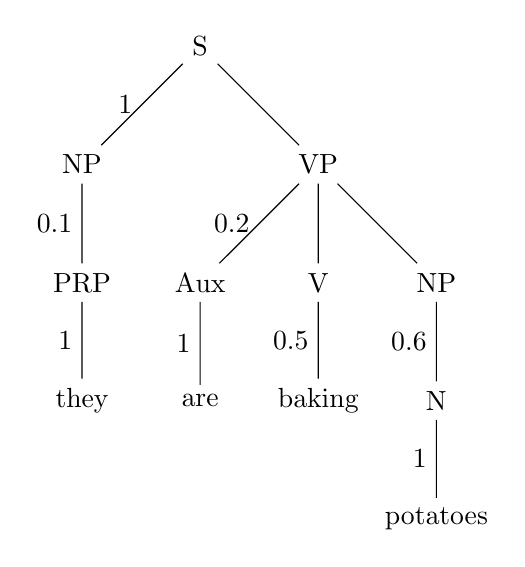
\begin{tikzpicture}
    [ level distance=1.5cm
    , level 1/.style={sibling distance=3cm}
    , level 2/.style={sibling distance=1.5cm}
    ]
  \node {S}
    child {node {NP}
      child {node {PRP}
        child {node {they}
          edge from parent {node[left] {1}}
        }
        edge from parent {node[left] {0.1}}
      }
      edge from parent {node[left] {1}}
    }
    child {node {VP}
      child {node {Aux}
        child {node {are}
          edge from parent {node[left] {1}}
        }
        edge from parent {node[left] {0.2}}
      }
      child {node {V}
        child {node {baking}
          edge from parent {node[left] {0.5}}
        }
      }
      child {node {NP}
        child {node {N}
          child {node {potatoes}
            edge from parent {node[left] {1}}
          }
          edge from parent {node[left] {0.6}}
        }
      }
    }
  ;
  \end{tikzpicture}

  \[
    \begin{aligned}
        &P[tags, words = \{they, are, baking, potatoes\}]\\
      = &P[S \rightarrow NP\ VP] \cdot P[NP \rightarrow PRP] \cdot P[VP \rightarrow Aux\ V\ NP] \cdot P[PRP \rightarrow they]\\
        &\cdot P[Aux \rightarrow are] \cdot P[V \rightarrow baking] \cdot P[NP \rightarrow N] \cdot P[N \rightarrow potatoes]\\
      = &1 \cdot 0.1 \cdot 0.2 \cdot 1 \cdot 1 \cdot 0.5 \cdot 0.6 \cdot 1\\
      = &0.006
    \end{aligned}
  \]

  second parse:\\
  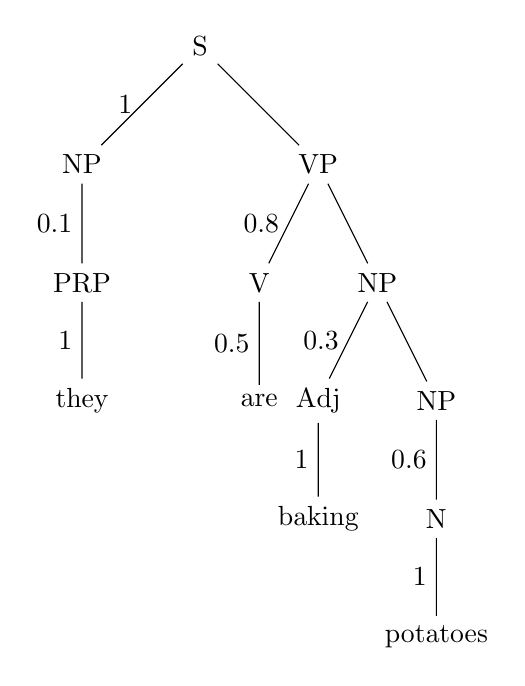
\begin{tikzpicture}
    [ level distance=1.5cm
    , level 1/.style={sibling distance=3cm}
    , level 2/.style={sibling distance=1.5cm}
    ]
  \node {S}
    child {node {NP}
      child {node {PRP}
        child {node {they}
          edge from parent {node[left] {1}}
        }
        edge from parent {node[left] {0.1}}
      }
      edge from parent {node[left] {1}}
    }
    child {node {VP}
      child {node {V}
        child {node {are}
          edge from parent {node[left] {0.5}}
        }
        edge from parent {node[left] {0.8}}
      }
      child {node {NP}
        child {node {Adj}
          child {node {baking}
            edge from parent {node[left] {1}}
          }
          edge from parent {node[left] {0.3}}
        }
        child {node {NP}
          child {node {N}
            child {node {potatoes}
              edge from parent {node[left] {1}}
            }
            edge from parent {node[left] {0.6}}
          }
        }
      }
    }
  ;
  \end{tikzpicture}
  \[
    \begin{aligned}
        &P[tags, words = \{they, are, baking, potatoes\}]\\
      = &P[S \rightarrow NP\ VP] \cdot P[NP \rightarrow PRP] \cdot P[VP \rightarrow V\ NP] \cdot P[PRP \rightarrow they]\\
        &\cdot P[V \rightarrow are] \cdot P[NP \rightarrow Adj\ NP] \cdot P[Adj \rightarrow baking] \cdot P[NP \rightarrow N] \cdot P[N \rightarrow potatoes]\\
      = &1 \cdot 0.1 \cdot 0.8 \cdot 1 \cdot 0.5 \cdot 0.3 \cdot 1 \cdot 0.6 \cdot 1\\
      = &0.0072
    \end{aligned}
  \]
\end{solution}

\subsection*{(b)}

\begin{solution}
  \

  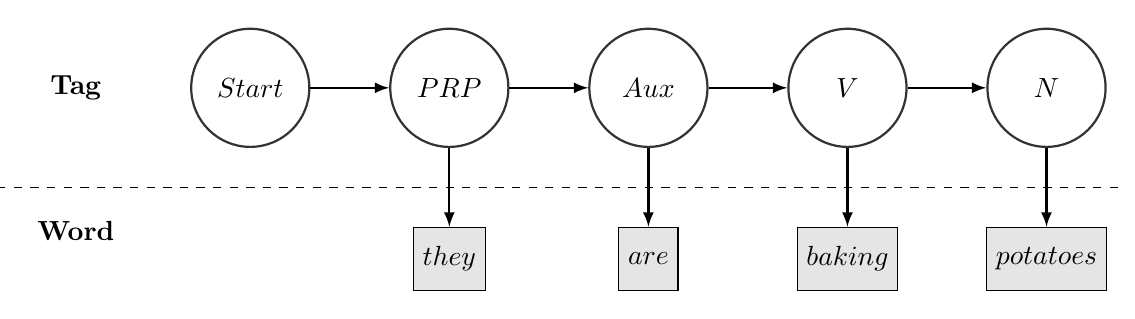
\begin{tikzpicture}
    \node[box,draw=white!100] (Latent) {\textbf{Tag}};
    \node[main] (Start) [right=of Latent] {$Start$};
    \node[main] (L1) [right=of Start] {$PRP$};
    \node[main] (L2) [right=of L1] {$Aux$};
    \node[main] (L3) [right=of L2] {$V$};
    \node[main] (Lt) [right=of L3] {$N$};
    \node[box,fill=black!10] (O1) [below=of L1] {$they$};
    \node[box,fill=black!10] (O2) [below=of L2] {$are$};
    \node[box,fill=black!10] (O3) [below=of L3] {$baking$};
    \node[box,fill=black!10] (Ot) [below=of Lt] {$potatoes$};
    \node[box,draw=white!100,below=of Latent] (Observed) {\textbf{Word}};

    \path (Start) edge [connect] (L1)
          (L1) edge [connect] (L2)
          (L2) edge [connect] (L3)
          (L3) edge [connect] (Lt);
    \path (L1) edge [connect] (O1)
          (L2) edge [connect] (O2)
          (L3) edge [connect] (O3)
          (Lt) edge [connect] (Ot);

    \draw [dashed, shorten >=-1cm, shorten <=-1cm]
        ($(Latent)!0.7!(Observed)$) coordinate (a) -- ($(Lt)!(a)!(Ot)$);
  \end{tikzpicture}

  \[
    \begin{aligned}
        &P[tags = \{PRP, Aux, V, N\}, words = \{they, are, baking, potatoes\}]\\
      = &P[tag = PRP | tag = Start] \cdot P[word = they | tag = PRP]\\
      \cdot &P[tag = Aux | tag = PRP] \cdot P[word = are | tag = Aux]\\
      \cdot &P[tag = V | tag = Aux] \cdot P[word = baking | tag = V]\\
      \cdot &P[tag = N | tag = V] \cdot P[word = potatoes | tag = N]\\
      = &0.006
    \end{aligned}
  \]

  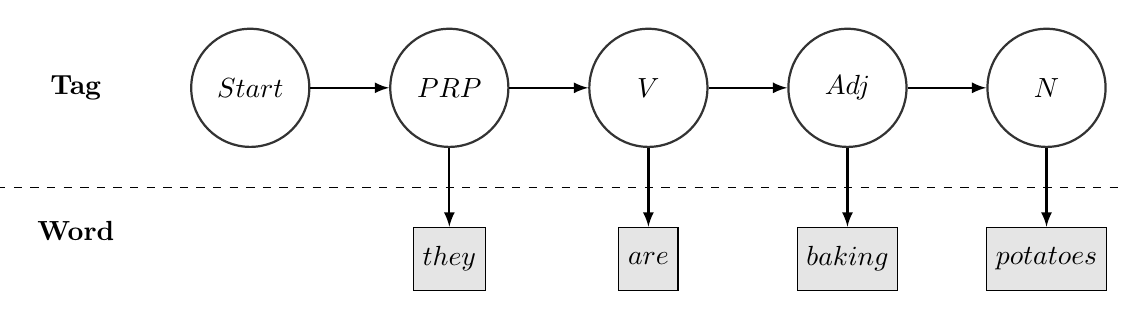
\begin{tikzpicture}
    \node[box,draw=white!100] (Latent) {\textbf{Tag}};
    \node[main] (Start) [right=of Latent] {$Start$};
    \node[main] (L1) [right=of Start] {$PRP$};
    \node[main] (L2) [right=of L1] {$V$};
    \node[main] (L3) [right=of L2] {$Adj$};
    \node[main] (Lt) [right=of L3] {$N$};
    \node[box,fill=black!10] (O1) [below=of L1] {$they$};
    \node[box,fill=black!10] (O2) [below=of L2] {$are$};
    \node[box,fill=black!10] (O3) [below=of L3] {$baking$};
    \node[box,fill=black!10] (Ot) [below=of Lt] {$potatoes$};
    \node[box,draw=white!100,below=of Latent] (Observed) {\textbf{Word}};

    \path (Start) edge [connect] (L1)
          (L1) edge [connect] (L2)
          (L2) edge [connect] (L3)
          (L3) edge [connect] (Lt);
    \path (L1) edge [connect] (O1)
          (L2) edge [connect] (O2)
          (L3) edge [connect] (O3)
          (Lt) edge [connect] (Ot);

    \draw [dashed, shorten >=-1cm, shorten <=-1cm]
        ($(Latent)!0.7!(Observed)$) coordinate (a) -- ($(Lt)!(a)!(Ot)$);
  \end{tikzpicture}
  \[
    \begin{aligned}
        &P[tags = \{PRP, V, Adj, N\}, words = \{they, are, baking, potatoes\}]\\
      = &P[tag = PRP | tag = Start] \cdot P[word = they | tag = PRP]\\
      \cdot &P[tag = V | tag = PRP] \cdot P[word = are | tag = V]\\
      \cdot &P[tag = Adj | tag = V] \cdot P[word = baking | tag = Adj]\\
      \cdot &P[tag = N | tag = Adj] \cdot P[word = potatoes | tag = N]\\
      = &0.0072
    \end{aligned}
  \]

  Here is my HMM:
  \begin{enumerate}
  \item tag-word transition distributions (the same as in PCFG):
    \begin{itemize}
    \item $P[word = they | tag = PRP] = 1$
    \item $P[word = are | tag = Aux] = 1$
    \item $P[word = baking | tag = V] = 0.5$, $P[word = are | tag = V] = 0.5$
    \item $P[word = potatoes | tag = N] = 1$
    \end{itemize}
  \item tag-tag transition distributions:
    \begin{itemize}
    \item $P[tag = PRP | tag = Start] = 1$
    \item $P[tag = Aux | tag = PRP] = 0.5$, $P[tag = V | tag = PRP] = 0.5$
    \item $P[tag = N | tag = V] = 0.5$, $P[tag = Adj | tag = V] = 0.5$
    \item $P[tag = V | tag = Aux] = 0.048$, $P[tag = PRP | tag = Aux] = 0.952$
    \item $P[tag = N | tag = Adj] = 0.0576$
    \item $P[tag = PRP | tag = N] = 1$
    \end{itemize}
  \end{enumerate}

\end{solution}

\subsection*{(c)}
\begin{prob}
  In general, is it possible to translate any PCFG into an HMM that produces the
  identical \textit{joint} probability P(tags, words) as PCFG (i.e. not just for
  a single sentence)? Explain how or why not. No formal proof is necessary.
  Hint: This has nothing to do with probabilities, but with language classes.
\end{prob}
\begin{solution}
  The hidden/latent state space in HMM can be formally described
  by a finite state machine which is strictly less expressive than pushdown
  automaton / context-free grammar in PCFG.
\end{solution}

\section*{Problem 2}

Consider the following probabilistic context free grammar.

\[
  \begin{aligned}
    S &\rightarrow NP\ VP &[1.0]\\
    NP &\rightarrow Adj\ NP &[0.3]\\
    NP &\rightarrow PRP &[0.1]\\
    NP &\rightarrow N &[0.6]\\
    VP &\rightarrow V\ NP &[0.8]\\
    VP &\rightarrow Aux\ V\ NP &[0.2]\\
    PRP &\rightarrow they &[1.0]\\
    N &\rightarrow potatoes &[1.0]\\
    Adj &\rightarrow baking &[1.0]\\
    V &\rightarrow baking &[0.5]\\
    V &\rightarrow are &[0.5]\\
    Aux &\rightarrow are &[1.0]\\
  \end{aligned}
\]

\subsection*{(a)}
\begin{prob}
  Using this grammar, show how the \textbf{Earley algorithm} would parse the
  following sentence.

  \textit{they are baking potatoes}

  Write down the complete parse chart.
  The chart should contain $n + 1$ entries where $n$ is the length of the
  sentence.
  Each entry $i$ should contain \textit{all} parser items generated by the
  parser that end in position $i$.
  You can ignore the probability for part (a).
\end{prob}

\end{document} 
